\section*{11. Optimization}
\begin{itemize}
    \item
        Convexity (geometric interpretation): $f$ is convex, if the line segment between $(x, f(x))$ and $(y, f(y))$ lies above the graph of $f$. $-f(x)$ is concave.
\end{itemize}
\subsection*{Unconstraint Optimization}
\begin{itemize}
    \item
        Assume convex function $f: \mathbb{R} \rightarrow \mathbb{R}$ that is twice differentiable
    \item
        The unconstraint optimization problem is just the solution of the minimization problem $x^* = \underset{x}{argmin} f(x)$, where $x^*$ denotes the optimal value
\end{itemize}
\subsection*{Descent Methods}
\begin{itemize}
    \item
        Iteration scheme which produces sequence of estimates:
        $$x^{(k+1)} = g(x^{(k)}) = x^{(k)} + t^{(k)} \Delta x^{(k)}$$
        where $\Delta x^{(k)}$ is the search direction and $t^{(k)}$ denotes the step length and where we expect $f(x^{(k+1)} < f(x^{(k)})$, except when $x^{(k+1)} = x^{(k)} = x^*$
    \begin{lstlisting}[mathescape]
    Input: function $f$, initial estimate $x^{(0)}$
    Initialize: $k=0$
    repeat
        Select (or compute) descent direction
        Line search (1-D optimization)
            $t^{(k)} = \underset{t \geq 0}{argmin} f(x^{(k)}) + t \cdot \Delta x^{(k)}$
        Update
            $x^{(k+1)} = x^{(k)} + t^{(k)} \Delta x^{(k)}$
        $k = k+1$
    until $\norm{x^{(k)} - x^{(k-1)}} < \epsilon$
    Output: $x^{(k)}$
    \end{lstlisting}
    \item
        Finding exact optimal solution $t^{(k)}$ is rarely used. Alternative: Backtracking Line Search, ...
\end{itemize}
\subsubsection*{Gradient Descent Methods} 
\begin{itemize}
    \item
        Natural choice of the search direction is the negative gradient
        $$\Delta x^{(k)} = - \nabla f(x^{(k)})$$
    \item
        Rule of thumb: steepest descent direction
\end{itemize} 
\subsubsection*{(Normalized) Steepest Descent Methods}
\begin{itemize}
    \item
        We search for the unit vector that shows the largest decrease in the linear appoximation of f:
        $$ \Delta x = \underset{u}{argmin}\{\nabla f(x)^T u; \norm{u}_p = 1\}$$ $(uv = |u||v|cos(\theta))$
    \item
        $L_1$-norm: selects component of $\nabla f(x)$ with maximum value (coordinate descent)
        $$ \Delta x = -sgn(\ffrac{\partial}{\partial x_i} f(x)) e_i$$
    \item
        $L_2$-norm:
        $$ \Delta x = - \nabla f(x)$$
    \item
        So gradient and coordinate descent are special cases of steepest descent methods
    \item
        $L_p$-norm:
        $$ \Delta x = - P^{-1} \nabla f(x)$$
\end{itemize}

\begin{figure}[H]
    \centering
    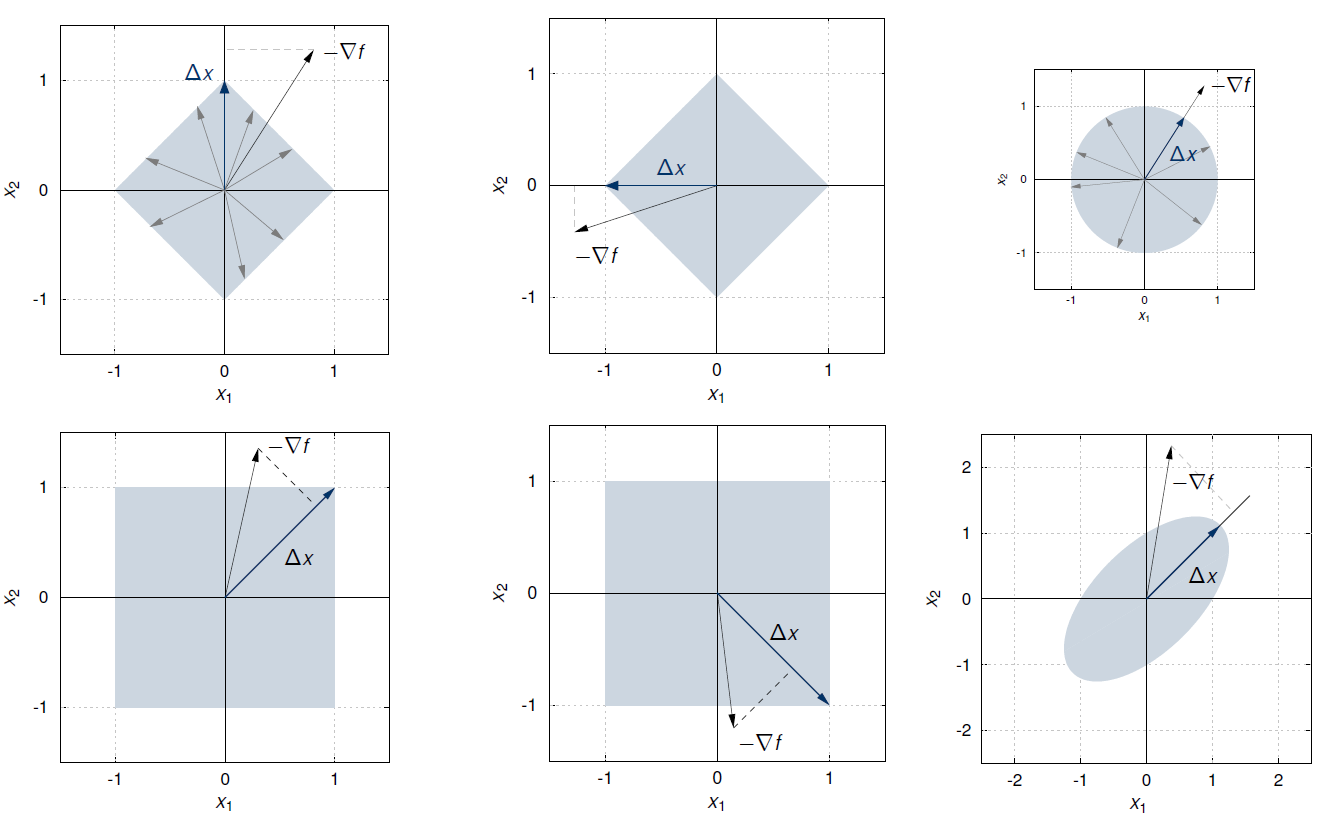
\includegraphics[scale=0.4]{figures/steep}
\end{figure}

\subsection*{Newton's Method}
\begin{itemize}
    \item
        Idea: Select a point, compute the minimum of the second order Taylor approximation
    \item
        Second order Taylor:
        $$f(x + \Delta x) = f(x) + \nabla f(x)^T \Delta x + \ffrac{1}{2} \Delta x^T (\nabla^2 f(x)) \Delta x$$
    \item
        Now select $\Delta x$ such that 
        $$\nabla \{f(x) + \nabla f(x)^T \Delta x + \ffrac{1}{2} \Delta x^T (\nabla^2 f(x)) \Delta x\} = 0$$
    \item
        The gradient is
        $$\nabla f(x) + \nabla^2 f(x) \Delta x = 0$$
        and thus
        $$\Delta x = -(\nabla^2 f(x))^{-1} \nabla f(x)$$
        \begin{figure}[H]
            \centering
            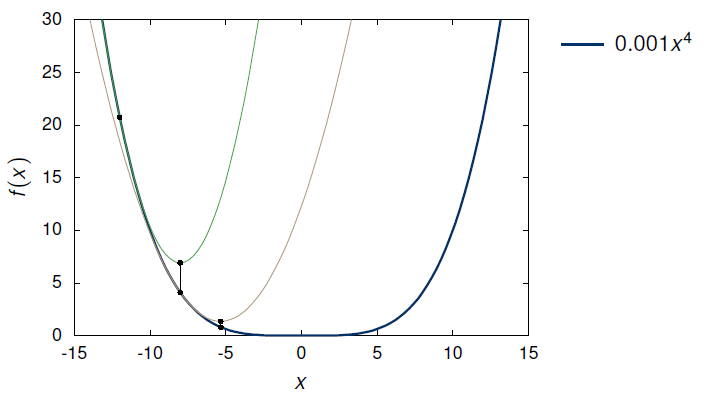
\includegraphics[scale=0.8]{figures/newton}
        \end{figure}

\end{itemize}

